For the following questions, refer to the microcontroller block diagram below. It is comprised of four main blocks (CPU, Data storage, Instruction storage, and Peripherals) and three buses (Address, Data, and Control).
\begin{center}
  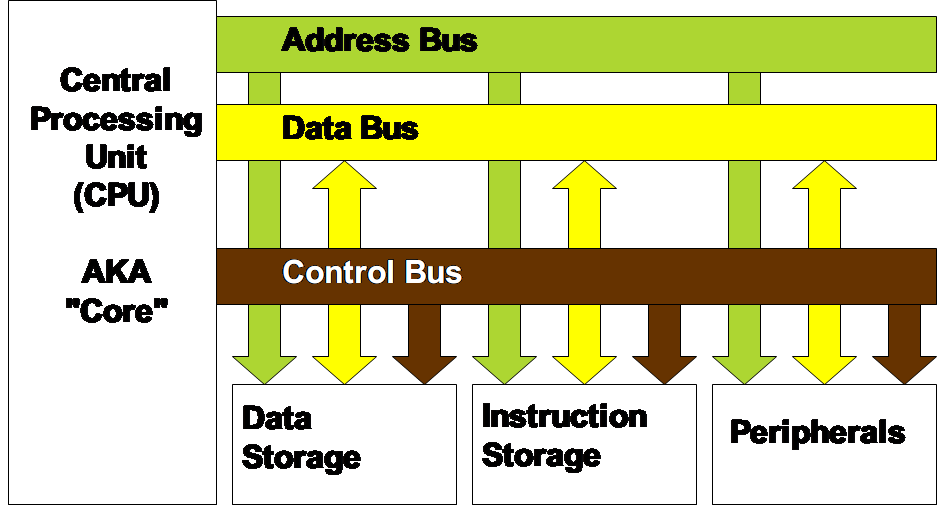
\includegraphics[width=.7\textwidth]{\QuestionBaseDir/figures/MCUBlockDiagram.png}
\end{center}

\begin{question}{q1-a}
  Which block would contain timers? Why?
  \AMCOpen{lines=3,
    dots=false,  }{
\wrongchoice[W]{w}\scoring{0}
\wrongchoice[P]{p}\scoring{1}
\correctchoice[C]{c}\scoring{2}}
\end{question}
% ANSWER: Timers are contained in the peripheral block. This block contains extra items that extend what the CPU can do.

\begin{question}{q1-b}
  Which block would contain ALU? Why?
  \AMCOpen{lines=3,
    dots=false,  }{\wrongchoice[W]{w}\scoring{0}\wrongchoice[P]{p}\scoring{1}\correctchoice[C]{c}\scoring{2}}
\end{question}
% ANSWER: The CPU block contains the ALU. This is where all basic processing is done.

\begin{question}{q1-c}
  Which block is most likely to have non-volatile memory? Why?
  \AMCOpen{lines=3,
    dots=false,  }{\wrongchoice[W]{w}\scoring{0}\wrongchoice[P]{p}\scoring{1}\correctchoice[C]{c}\scoring{2}}
\end{question}
% ANSWER:Instruction storage. This stores code that needs to be retained between power cycles.

\begin{question}{q1-d}
  Which block contains the logic to decode what an instruction actually does? Why?
  \AMCOpen{lines=3,
    dots=false,  }{\wrongchoice[W]{w}\scoring{0}\wrongchoice[P]{p}\scoring{1}\correctchoice[C]{c}\scoring{2}}
\end{question}
% ANSWER: CPU. CPU block's core function is to retrieve, decode and execute instructions

\begin{question}{q1-e}
  How would the block diagram differ for a microprocessor?
  \AMCOpen{lines=3,
    dots=false,  }{\wrongchoice[W]{w}\scoring{0}\wrongchoice[P]{p}\scoring{1}\correctchoice[C]{c}\scoring{2}}
\end{question}
% ANSWER: A microprocessor is only the CPU. Everything else requires external ICs.

